% !TEX root = ../main.tex
\chapter{Results and Discussion}\label{ch:results}
This chapter will look into the results we gained after running the analysis across all opponents.
Details of the distribution of the results and basic output from the computation are given in section~\ref{sec:descriptive_data}.

The analysis performed in this chapter contains data for opponents listed in Appendix~\ref{apndx:opponents}.
Opponents without results due to being incomplete are all the Long Run Time (LRT) strategies.
As these become available they will be added to the analysis.
% TODO: add the extra data if it becomes available

Each opponent was submitted to the compute engine using the standard analysis factory class \mintinline{python}{AnalysisRun}, shown in Figure~\ref{apcode:AnalysisRun.py}, using native multi-threading on a Linux OS to improve individual opponent analysis run times and the overall scalability of the project.
We ran the code over a period of days resulting in 200+ output files of data which could then be analysed.

\section{Resulting Data}\label{sec:descriptive_data}
The data we generated from the final analysis contained 760 of the 959 opponents we set out to analyse.
Figure~\ref{table:data_dump} shows a raw data head from the output of the $\phi$ opponent.

\begin{table*}[ht]
    \centering
    \begin{tabular}{ccccccccc}
        \toprule
        gen & score mean & score median & score var & score range & best score & best sequence &  name & seed \\
        \midrule
        1 & 2.90966 & 3.0575 & 1.665496 & 4.985 & 5.0 & DDD\ldots & $\phi$ & 0 \\
        2 & 4.79004 & 4.9250 & 0.420476 & 2.275 & 5.0 & DDD\ldots & $\phi$ & 0\\
        3 & 4.79352 & 4.97 & 0.489173 & 2.185 & 5.0 & DDD\ldots & $\phi$ & 0\\
        4 & 4.81386 & 5 & 0.460776 & 2.2 & 5.0 & DDD\ldots & $\phi$ & 0\\
        5 & 4.81826 & 5 & 0.479307 & 2.18 & 5.0 & DDD\ldots & $\phi$ & 0\\
        6 & 4.83508 & 5 & 0.430063 & 2.03 & 5.0 & DDD\ldots & $\phi$ & 0\\
        \ldots & \ldots & \ldots & \ldots & \ldots & \ldots & \ldots & \ldots & \ldots\\        
        \bottomrule
    \end{tabular}
    \caption{Raw data from \mintinline{python}{AnalysisRun.py} output file}\label{table:data_dump}
\end{table*}

The data collected was, for each of the strategies, merged and collated with metadata to form an analysis table which was then processed.
This metadata included player classifiers as given in the Axelrod library, generated values from fields in Table~\ref{table:data_dump} and information generalizing stochastic players to their original base player before seeding.
Table~\ref{table:meta_data} shows the first few rows of this information.

\begin{table*}[ht]
    \centering
    \begin{tabular}{cccccccc}
        \toprule
        base & stochastic & memory depth & makes use of & score bin & start move & blocks & mean block length\\
        \midrule
        $\phi$ & False & inf & \mintinline{python}{set()} & very high &  $D$ & 1 & 200\\

        $\pi$ & False & inf & \mintinline{python}{set()} & very high &  $D$ & 1 & 200\\

        $e$ & False & inf & \mintinline{python}{set()} & very high &  $D$ & 1 & 200\\

        ALLCorALLD & True & 1 & \mintinline{python}{set()} & very low/high\footnote{Stochastic opponents can have different score bins depending on the seed.} &  $D$ & 1 & 200\\

        Adaptive & False & inf & \mintinline{python}{'game'} & very high &  $C$ & 2 & 100\\

        \ldots & \ldots & \ldots & \ldots & \ldots & \ldots & \ldots & \ldots\\    
        \bottomrule
    \end{tabular}
    \caption{Metadata which was merged to Table~\ref{table:data_dump} during analysis; joined base on name.}\label{table:meta_data}
\end{table*}

When analysing the overall best sequences for each opponent we can pick out some interesting and descriptive data.
The distribution on best scores are showing in Figure~\ref{fig:best_score_hist}, its kernel density estimate (KDE) \cite{tukey1977exploratory} exaggerates that fact we have a skew towards the higher scores with a fat tail on 4.5 to 5.
This shows we can average a score higher than 3.0 against the majority of opponents per turn.
From this we can infer that there is a way of outplaying many of the opponents in the Axelrod Library (i.e. we can perform better than a game where both players would have an avg score of $3.0$ from mutual cooperations).
If there is a way of identifying an opponent then we would be able to tip the scales in a tournament in our favour by playing the sequences shown.

\begin{figure}[ht]
    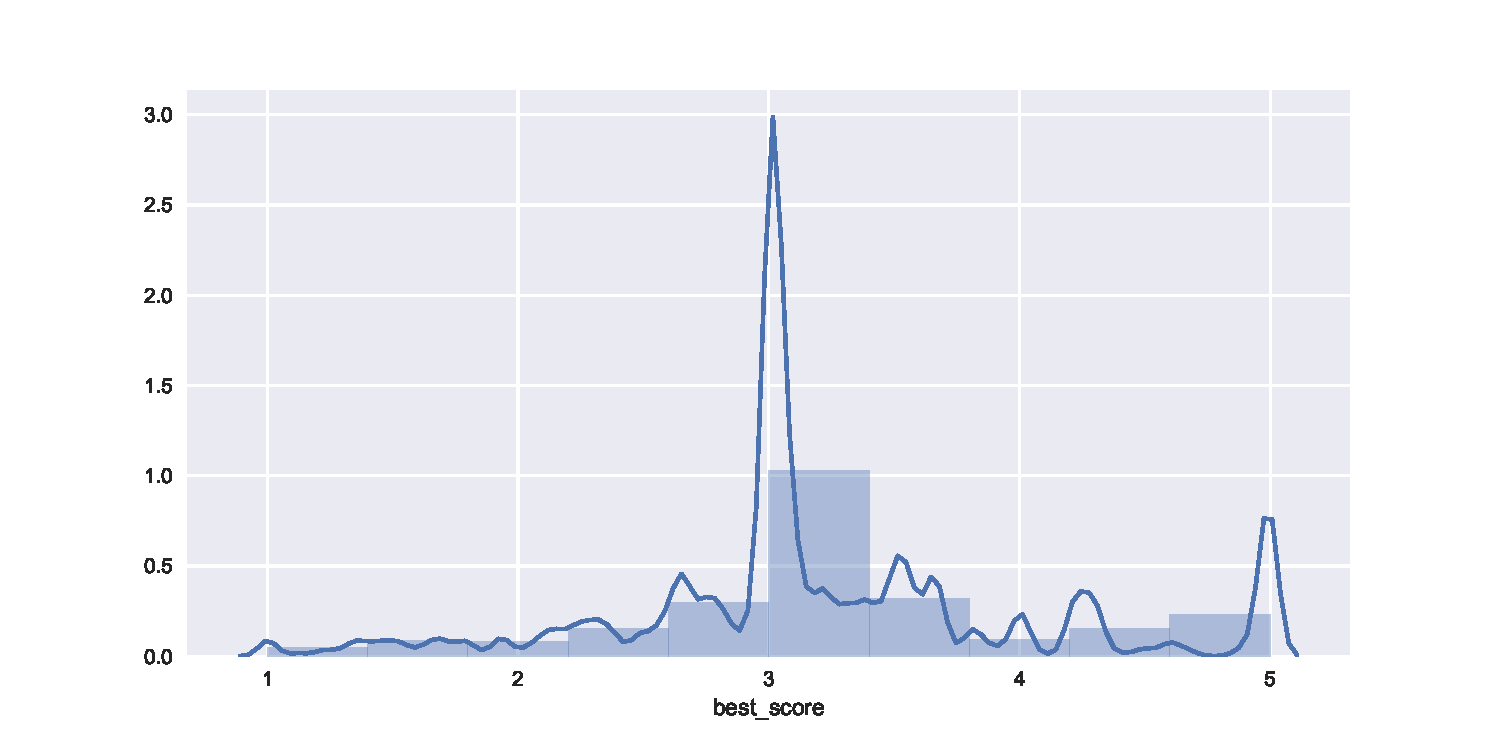
\includegraphics[width=0.95\textwidth, center]{./img/descriptive/best_score_hist.pdf}
    \caption{A histogram showing the distribution of best scores with overlaid KDE}\label{fig:best_score_hist}
\end{figure}

Figure~\ref{fig:cor_plot} shows patterns related to how the number of blocks within a sequence changes depending on score, opponent type and start move.
In the left plot, solution sequences starting with a defection lead to 3 groupings; low block number, between 50 \& 125 blocks and near 200.
This pattern has little information that describes the relationship between the solutions, but there could be an underlying reason in the make-up of an opponent which describes the groupings.
All 3 contain both stochastic and non stochastic and have a wide range of scores.
Starting with a cooperation shows a trend for non stochastic opponents; ignoring the near totalities on the far right shows a linear trend from 0 to 200 blocks as the score increases.
This trend describes that, for non stochastic opponents, there are complicated solutions that score us more than simple solutions for particular opponents.
It shows evidence that if a non stochastic opponent is more complicated in its solution, we can do better than if it is simple; for example, the solution for Tit For Tat is $C199,1$ which scores 3.01 whereas Adaptive Pavlov 2011 has the alternator solution $C1,1,1,1,\ldots$ and scores 3.97.
This does not hold for stochastic opponents as, for example, ZD Extort with seed 0 has the solution sequence $D4,5,1,9,1,41,1,42,1,90,$ and only scored a 1.355.

By looking into the distributions of best scores and the make up of solutions we are showing 2 things.
That most opponents can be outplayed; we are able to score higher than an average of 3 per turn over the course of the game and hence, by the definition of the prisoners dilemma, defiantly come out with a higher score than our opponent.
And that solution sequences are varied and there is little correlation between the complexity of a solution and the best score we can achieve. 

\begin{figure}[ht]
    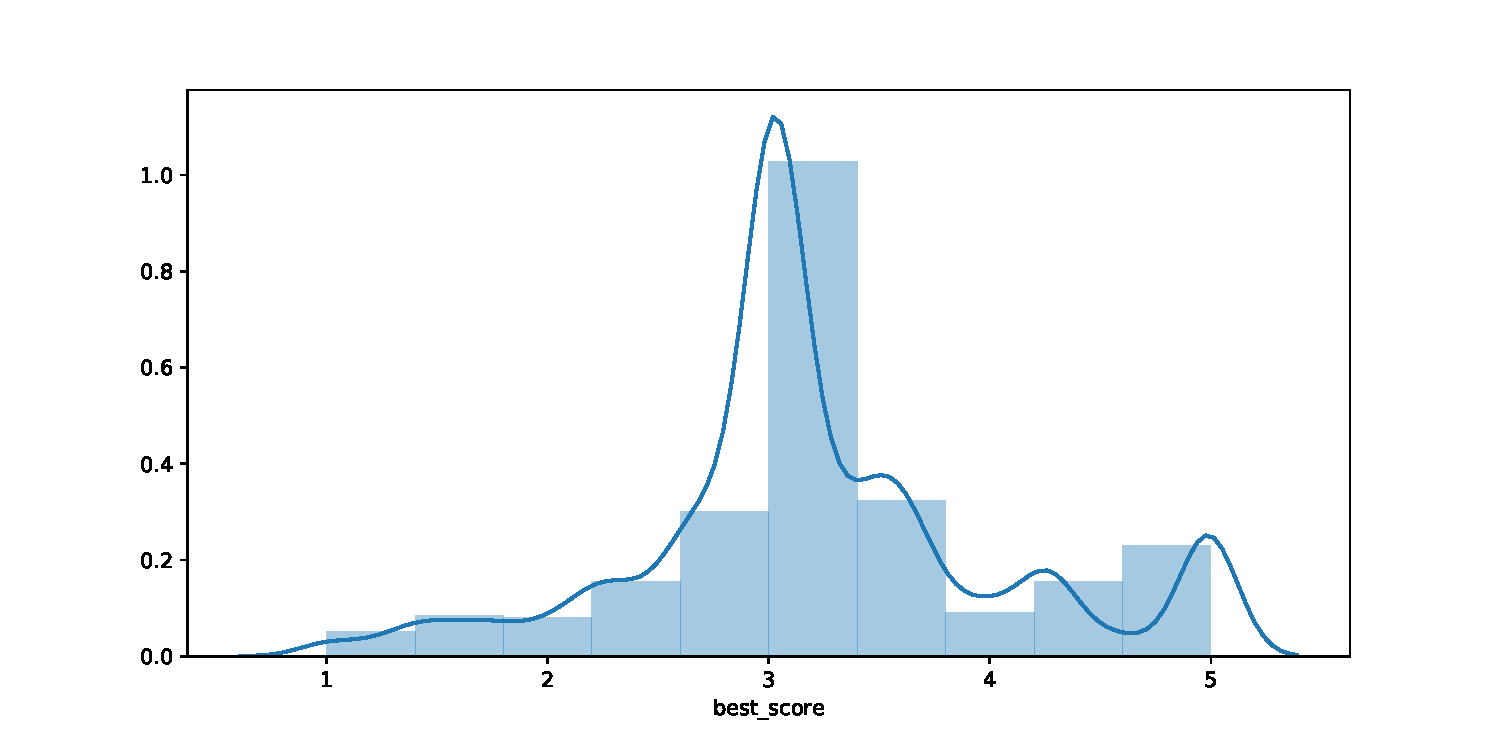
\includegraphics[width=0.95\textwidth, center]{./img/descriptive/cor_plot.pdf}
    \caption{A joint plot of best score vs number of blocks coloured by stochastic boolean}\label{fig:cor_plot}
\end{figure}

\section{Solution Distance Matrices}\label{sec:distance_matracies}
The first avenue of analysis, after constructing descriptive data, was to look at the relationship best response sequences have with each other.
A distance matrix shows how much  sequence for one opponent differs from every other, if 2 sequences are similar with respect to the distance function then they will score lower than 2 sequences that are more distinct.

In each matrix we order the opponents, $S_(O_i)$, by the score of their sequences\footnote{See section~\ref{sec:notation} for explanations of notation.} so that the order is now $f(S_{O_0}) \ge f(S_{O_1}) \ge \ldots \ge f(S_{O_n})$. but we will shorten this notation $S_{O_i}$ to $S_{i}$ for simplicity.
The best response sequence for the $i$th opponent, $S_i$ vs the best response sequence for the $j$th, $S_j$ is scored using our distance function, for example $d(S_0,S_n)$ is the distance between the best and worst scoring sequences respectively.
The Matrix itself will be symmetric down the diagonal, so looking across rows vs columns tends to make more logical sense; the top rows are the highest scoring best response sequences, and the lower rows the worse scoring sequences.

There were two distance measures considered: Hamming Distance and Cosine Distance.

\paragraph{Hamming Distance}\cite{norouzi2012hamming}
$$d(S_i,S_j) = S_i \cdot S_j^T $$
This corresponds to 
$$ 1-\frac{\sum^n_{i,j=0}\delta_{ij}}{n}\text{ where } \delta_{ij} = \begin{cases} 
    1 & i=j \\
    0 & i\ne j 
\end{cases} $$

The Hamming Distance represents the count of the elements that differ in any two sequences. 
A Hamming Distance will thus correspond to the number of places we have to play different moves against opponents to get out best score. 
Figure~\ref{fig:dist_ham} shows the matrix generated by the code in Figure~\ref{apcode:dist_matrix.py}.

By observing the graph row by row, we can build an idea of how similar each sequence is to the range of others.
The top section of the plot shows the best scoring sequences vs other high scoring sequences on the left, and vs the worse scoring sequences on the right. 
At the very top left there crossing dark and light columns, suggesting that there are lots of very similar or dissimilar solutions at the high vs high end of the score level.
As we move to  the high vs low scores there are larger blocks of dark red representing high dissimilarity.
This is shown again as we move to the bottom of the diagram.
The large blocks or red covering the bottom 100 or so rows show that the lowest scoring opponents have very different sequences to the higher scorers, but as a group of low scoring vs low scoring they are quite similar.

We can look into what distances we expect by trying to analyse how scored are formed.
The recording of an average score means that we can estimate the ratio of move combinations that formed a score because we know, if we are the first player, the pay offs for the combinations: $(C,C)=3$, $(C,D)=0$, $(D,C)=5$, $(D,D)=1$.
Thus we can assume scoring in the midrange ($3$ ish) means mostly cooperating, or a combination of $(C,D)$ and $(D,C)$, whereas at the high and low ends its more likely we are to be defecting.
This would mean when looking at the high vs low section and low vs high section of the graph we would expect a high level of similarity; $d(S_i,S_j)\approx 0$.
However this hypothesis is not supported; its clear there is a mix of distances because all 4 corners of the graph are not showing $d(S_i,S_j)\approx 0$. 

To understand why this disparity between expectation and result exists we can look at a visual representation of each of the strategies.
Figure~\ref{fig:sequence_plot_score} shows what the solution sequence looks like move by move, sorted by best scoring at the top of the left image moving down to worst scoring on the bottom of the right.
From this diagram it is clear that some of the predictions above were true; the very high and low scoring solutions are totalities of defections.
There is however much more noise for sequences at the top of the scoreboard, resulting in the large distances between the scores.

Figure~\ref{fig:sequence_plot_score} also shows some interesting results about picking up points in patterns.
Some opponents (aprox half way down on right image) work using ratios, we can trick them for half the game and take advantage for the remainder.
Others are much shorter term solution, alternating between $C$ and $D$ every other turn ($1/4$ down the left image).
When scoring in the mid range (bottom of right, top of left) there seems to be patterns too; totalities of $C$ are to be expected but there are some results that seem to be tricking an opponent for the first number of moved before defecting for the rest of the game.
At the higher score ranges there seems to be lots of noise, many of these opponents are rather complicated in their Strategy, the top 12 non totalities are listed below:

One final point regarding what Figure~\ref{fig:sequence_plot_score} shows is the effectiveness of the genetic algorithm.
From the theory of repeated games, an equilibria for the repeated game must end in an equilibria for the static game.
Hence for one of our solution sequences to be optimal the result must end in a $D$. 
This is true for all but $57$ of the solutions, meaning there is room for possible improvement in more than one result.
These sub optimal results were all stochastic.

\paragraph{Cosine Distance}\cite{bora2014effect}
The cosine of two vectors constructed by using the dot product formula as shown.
In our interpretation each dimension represents a sequence element so we are working in $\mathbb{R}^{200}$ with every value taking a $C:1$ a $D:0$.
Figure~\ref{fig:dist_cos} shows the distance matrix generated from the data files using code in Figure~\ref{apcode:dist_matrix.py}

$$ d(S_i,S_j) = \cos(\theta) = \frac{{S_i} \cdot {S_j}}{|| {S_i} || \; || {S_j} ||} $$

The Matrix for Cosine and Hamming are almost exactly similar, the only difference being the value of the distance between sequences.
This is due to the two measures being similar in their relationship of space~\cite{choi2010survey}.
We can conclude that there is no extra information shown in this diagram. 
\begin{figure}[ht]
    \centering
    \begin{minipage}{0.48\textwidth}
        \centering
        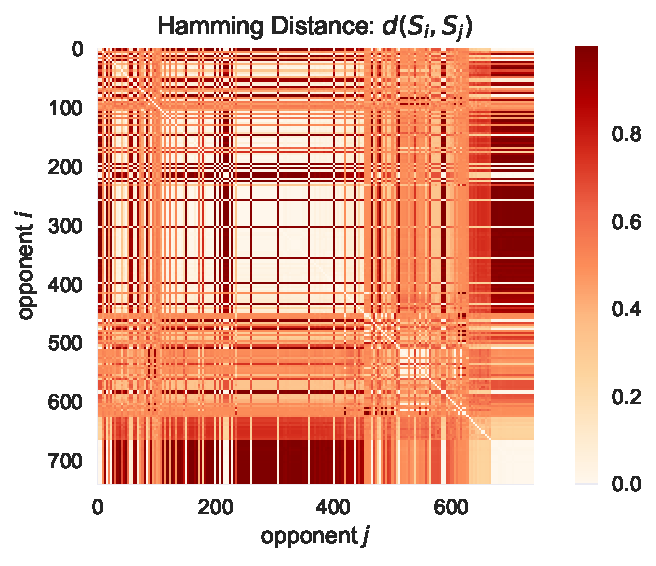
\includegraphics[width=1.0\textwidth, center]{./img/dist_matrix/dist_ham.pdf}
        \caption{Distance Matrix for Hamming Distance}\label{fig:dist_ham}
    \end{minipage}\hfill
    \begin{minipage}{0.48\textwidth}
        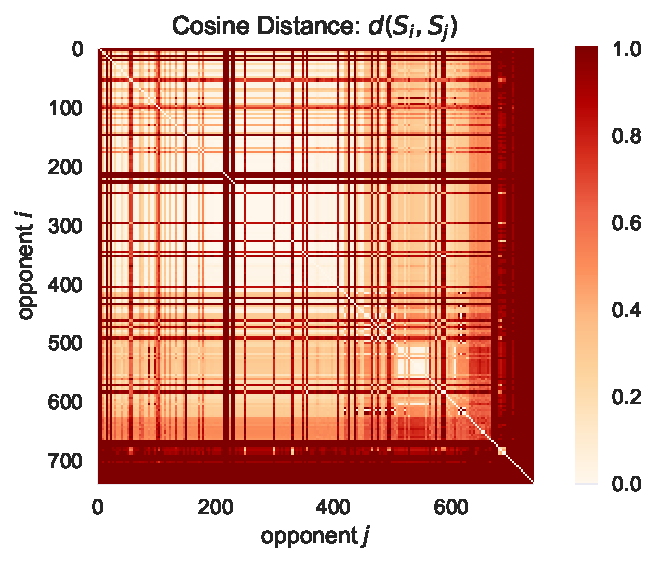
\includegraphics[width=1.0\textwidth]{./img/dist_matrix/dist_cos.pdf} 
        \caption{Distance Matrix for Cosine Distance}\label{fig:dist_cos}
    \end{minipage}
\end{figure}

\section{Solution Groups}\label{sec:solutionGroups}
\begin{figure}[ht]
    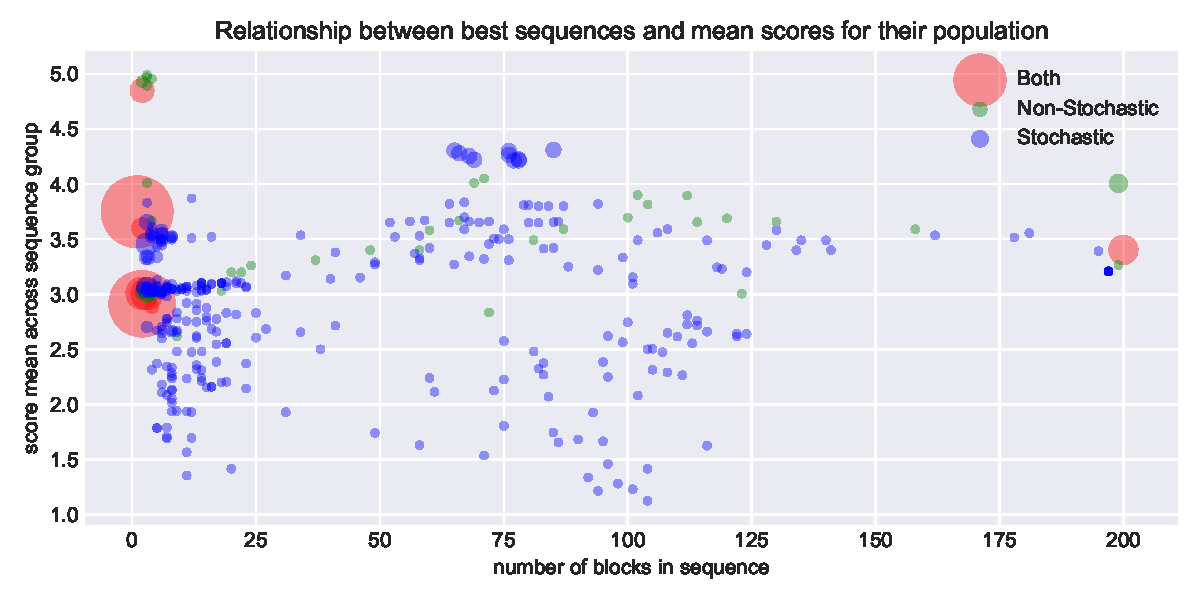
\includegraphics[width=0.95\textwidth, center]{./img/descriptive/sequence_scatter_colour.pdf}
    \caption{Trends for opponents grouped by their best sequence. Dot size represents the number of opponents in the group.}\label{fig:sequence_scatter}
\end{figure}

If we want to group opponents together, the most obvious way is to look at which opponents have have the same best score sequence.
Appendix~\ref{apndx:solutionGroups} has full details, and figure~\ref{fig:sequence_scatter} shows a plot of the trends. 
This figure shows an almost logarithmic/polynomial trend in score as the number of blocks in a sequence increases.
Below this trend there are also a group of stochastic opponents who dont seem to follow the pattern and form a group below this.
This could indicate that the trend only applies to specific strategies and that this grouping of stochastic opponents use more unforgiving approaches, such as the ZD Extort strategies.

\begin{figure}[ht]
    \centering
    \begin{minipage}{0.48\textwidth}
        \centering
        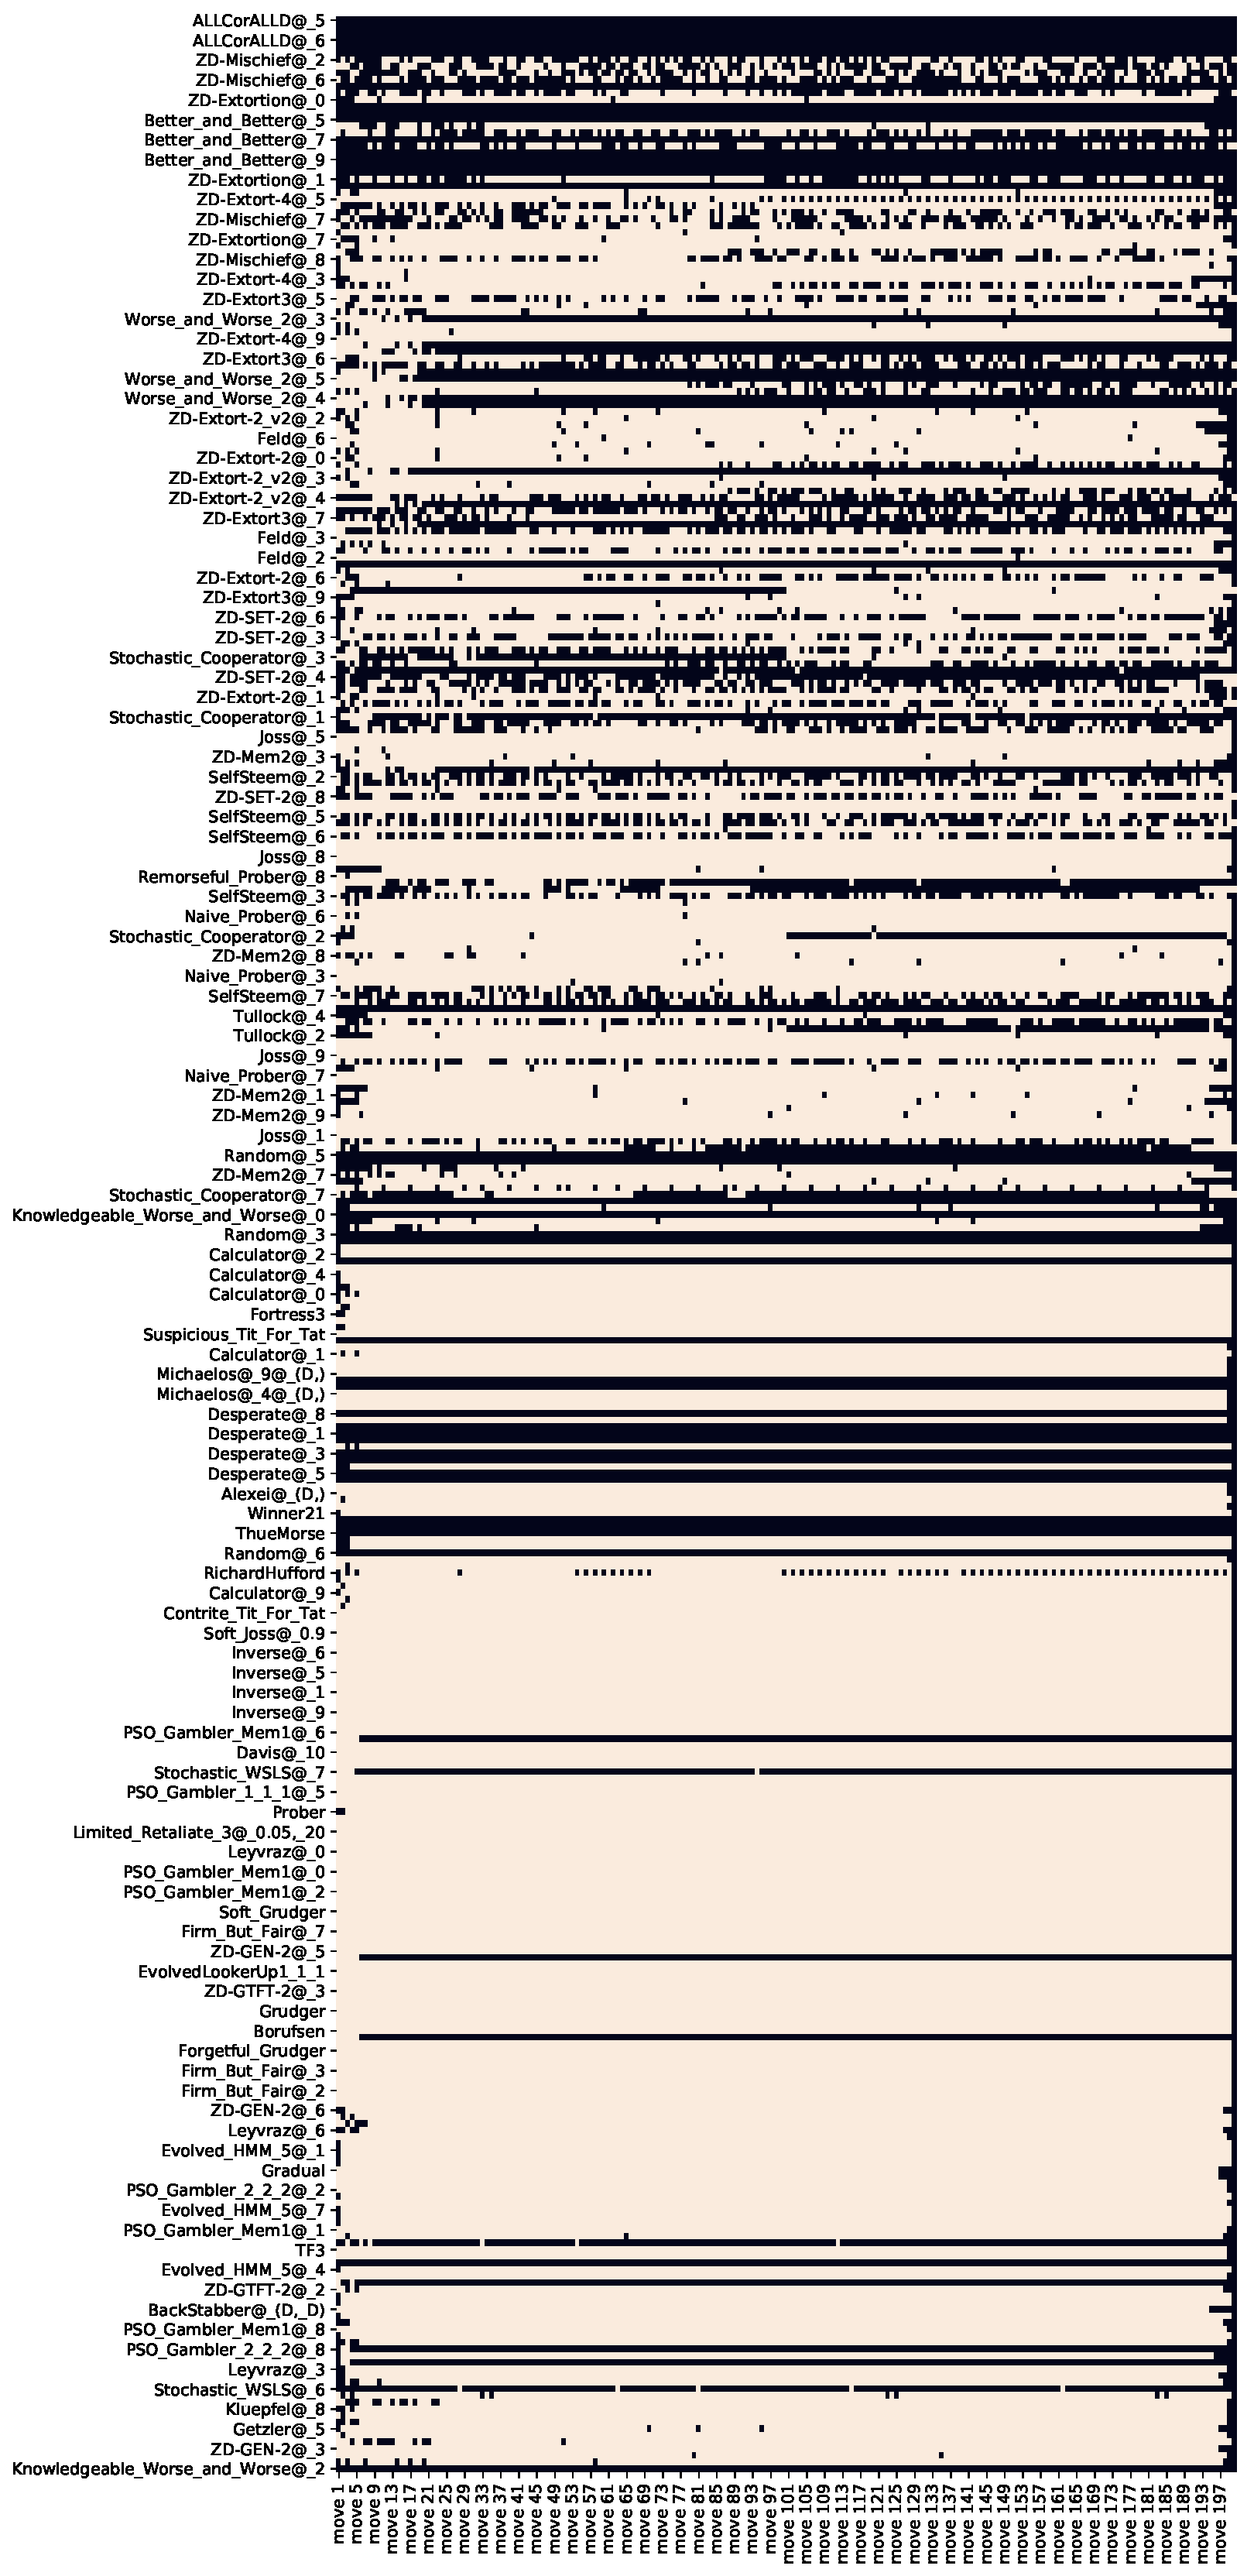
\includegraphics[width=1.0\textwidth, center]{./img/descriptive/sequence_plot_score_pt1.pdf}
    \end{minipage}\hfill
    \begin{minipage}{0.48\textwidth}
        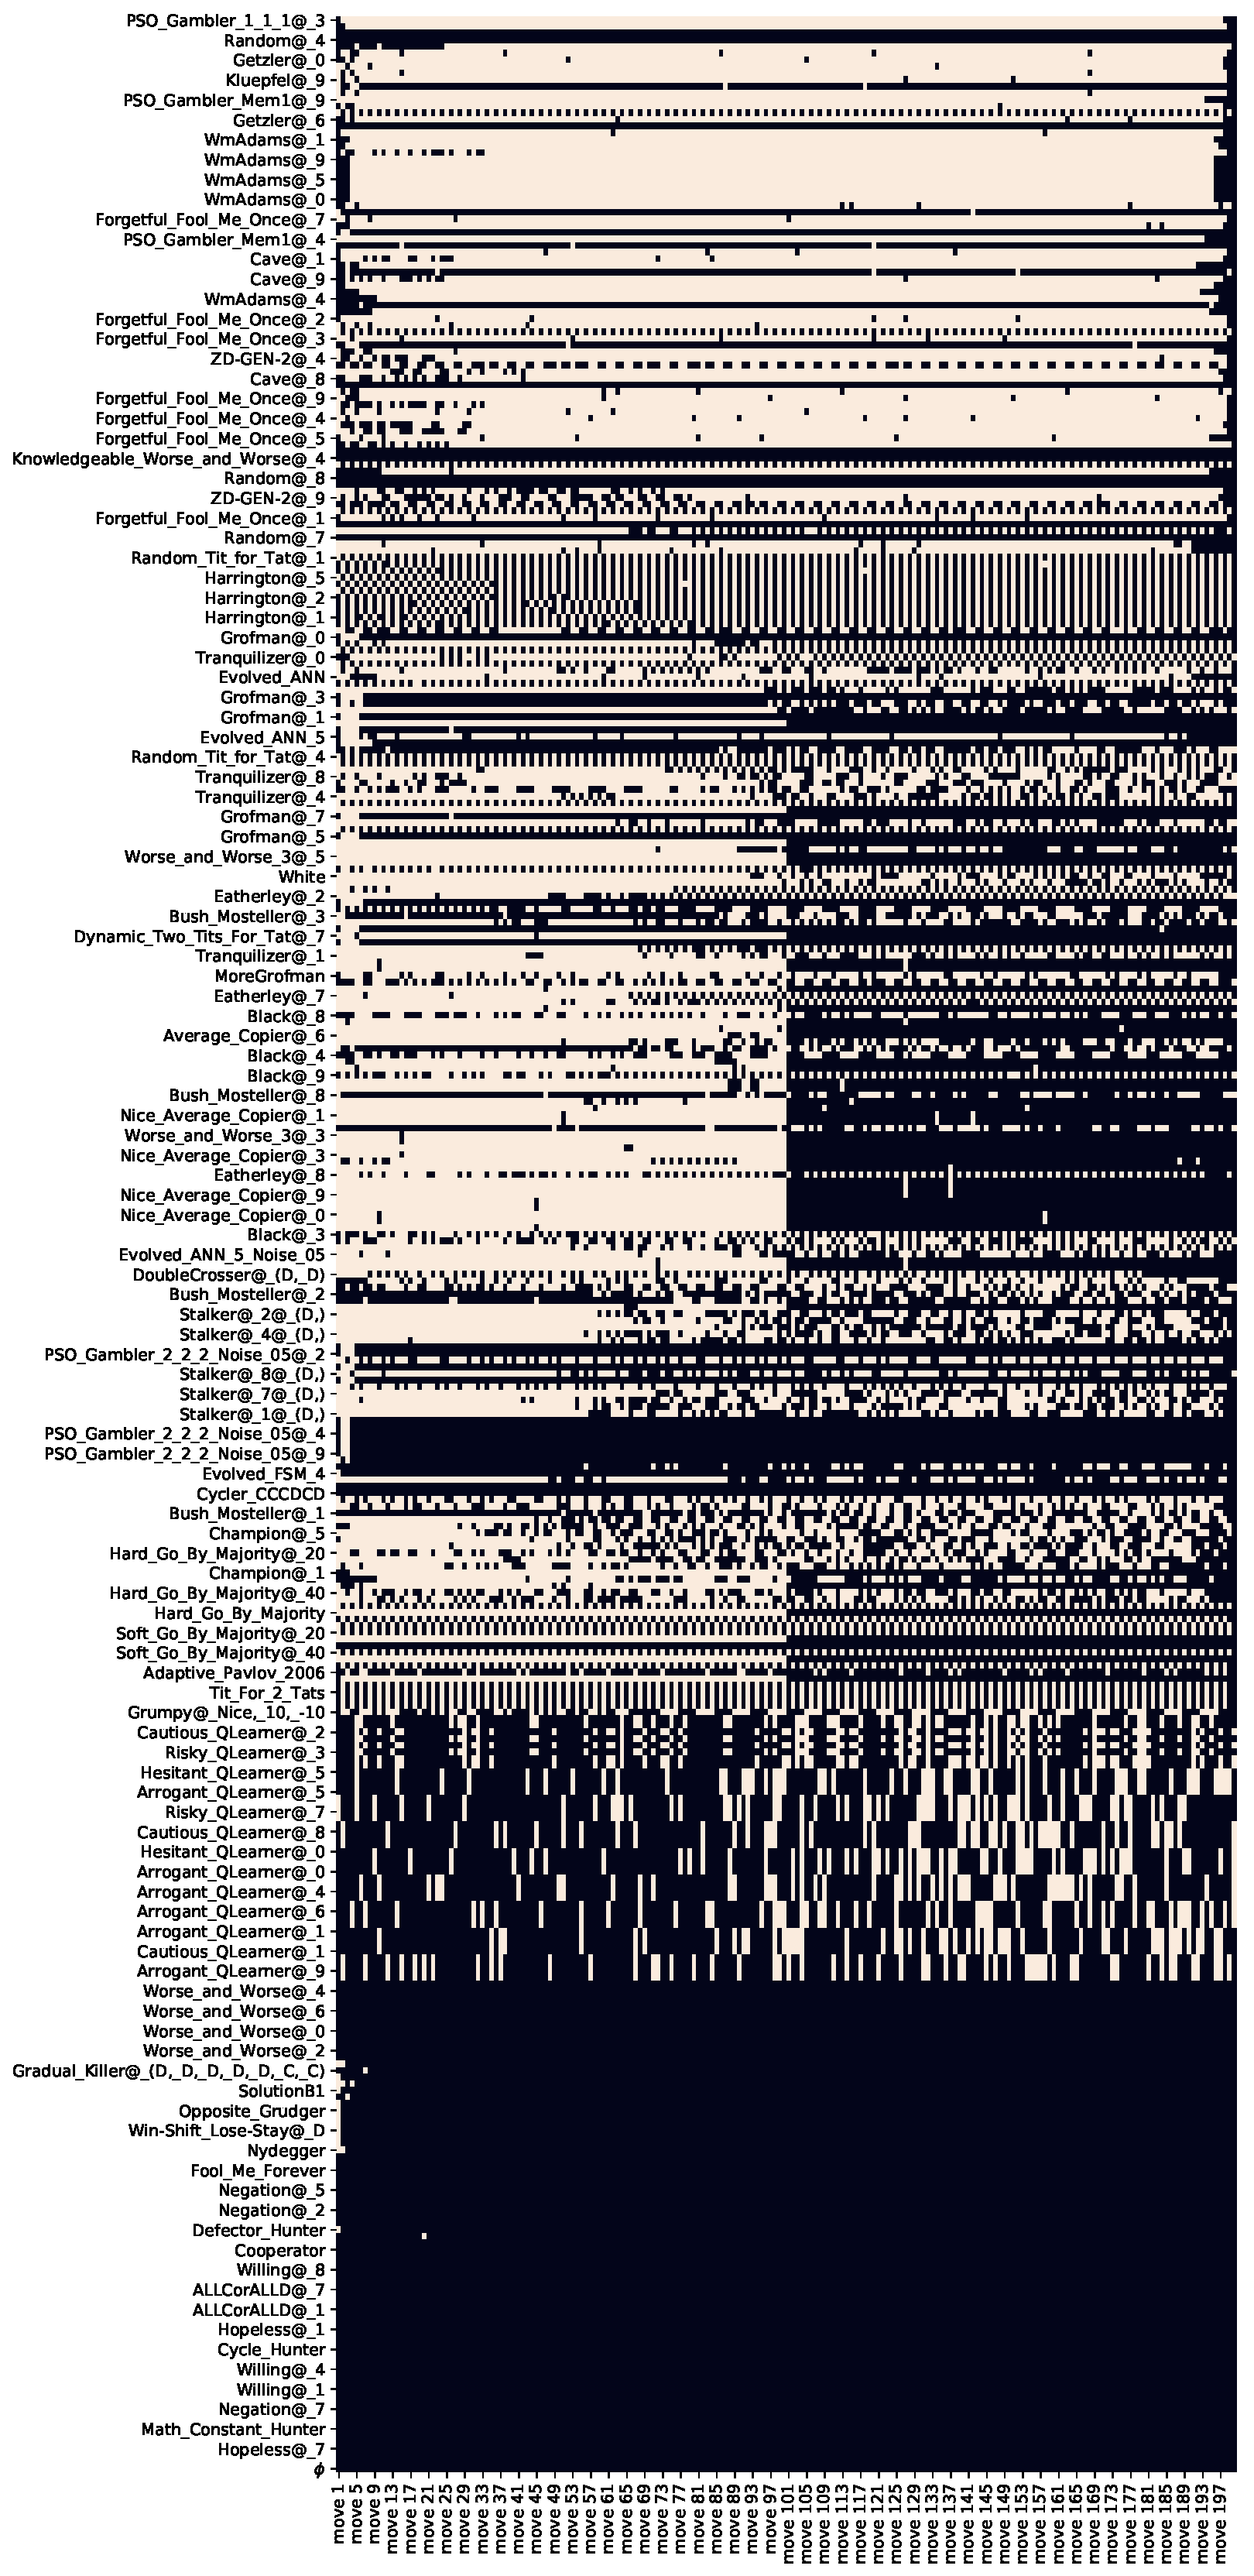
\includegraphics[width=1.0\textwidth, center]{./img/descriptive/sequence_plot_score_pt2.pdf}
    \end{minipage}
    \caption{Sequence Diagram, sorted by score; High: top left $\rightarrow$ bottom right: Low. $C$ is light and $D$ is Dark.
    \textit{NOTE: labels are not complete, approx 1 in 4 shown.}}\label{fig:sequence_plot_score}
\end{figure}

Figure~\ref{fig:sequence_plot_score} provides a visual representation of sequences so that identifying groups of equivalent or almost equivalent solution sequences is easy.
Families of similar solutions can be picked out, for example the Qlearners at the bottom right of the figure all have chunky sections to their solution sequences and are all grouped near one another, even though the hamming distance between any two in different families could be vastly different.
The bottom of the left figure shows many occurrences of the largest group, $C199,1$ with some that have similar strategies with larger tails.
Grouping strategies by their solution sequence seems to be very restrictive for providing relationships between strategies and solutions. 
It may be beneficial to apply some binary pattern recognition to the solutions, the solutions all seem quite chaotic that could have patterns in other areas of mathematics.

Of the likely sequences that were predicted to occur as solutions, as described in Section~\ref{sec:alteringinitialpopulation}, 29 of them appeared as actual solution sequences. 
This is shown below.

\begin{multicols}{3}
    \begin{itemize}
        \item  C199,1 with 96 opponents
	    \item  C198,2 with 21 opponents
	    \item  C196,4 with 3 opponents
	    \item  C194,6 with 1 opponent
	    \item  C193,7 with 2 opponents
	    \item  C100,100 with 8 opponents
	    \item  C5,195 with 3 opponents
	    \item  C2,1,1,196 with 1 opponent
	    \item  C2,198 with 2 opponents
	    \item  C1,1,1,1,\ldots with 17 opponents
	    \item  C1,1,1,197 with 1 opponent
	    \item  C1,2,1,196 with 1 opponent
	    \item  C1,199 with 11 opponents
	    \item  D1,198,1 with 21 opponents
	    \item  D1,196,3 with 1 opponent
	    \item  D1,194,5 with 2 opponents
	    \item  D1,4,195 with 4 opponents
	    \item  D1,3,196 with 4 opponents
	    \item  D1,2,197 with 9 opponents
	    \item  D2,197,1 with 3 opponents
	    \item  D2,196,2 with 2 opponents
	    \item  D2,195,3 with 1 opponent
	    \item  D2,194,4 with 2 opponents
	    \item  D2,193,5 with 1 opponent
	    \item  D2,1,197 with 1 opponent
	    \item  D3,196,1 with 4 opponents
	    \item  D3,194,3 with 1 opponent
	    \item  D3,192,5 with 8 opponents
	    \item  D200 with 113 opponents
    \end{itemize}
\end{multicols}
\section{Clustering Analysis}
Here we will look at ways of grouping opponents based on their best response sequences and what that means for scores and potential hidden relationships between strategies.
These clustering algorithms are not meant for predictive purposes and are all forms of unsupervised learning; there is not enough metadata present in each strategy definition to use as features for supervised prediction of our best response sequences.
These clustering algorithms come from the python library SciKit Learn~\cite{pedregosa2011scikit}.

\subsection{K Means clustering~\cite{bora2014effect}}\label{ssec:k_means}
Here we attempted to label k clusters depending on their parameters.
Nothing much was identified from the k means clustering data analysis, typically clusters were found to strongly correlate with parameters such as number of blocks or mean block length.
Figure~\ref{fig:k_means} shows the clustering for the most correlated variables in 3 dimensions.
Its clear that these clusters are layered over the number of blocks of the solutions sequence.
Section~\ref{sec:solutionGroups} looks in depth as to how opponents are distributed over the solution sequences. 

\begin{figure}[ht]
    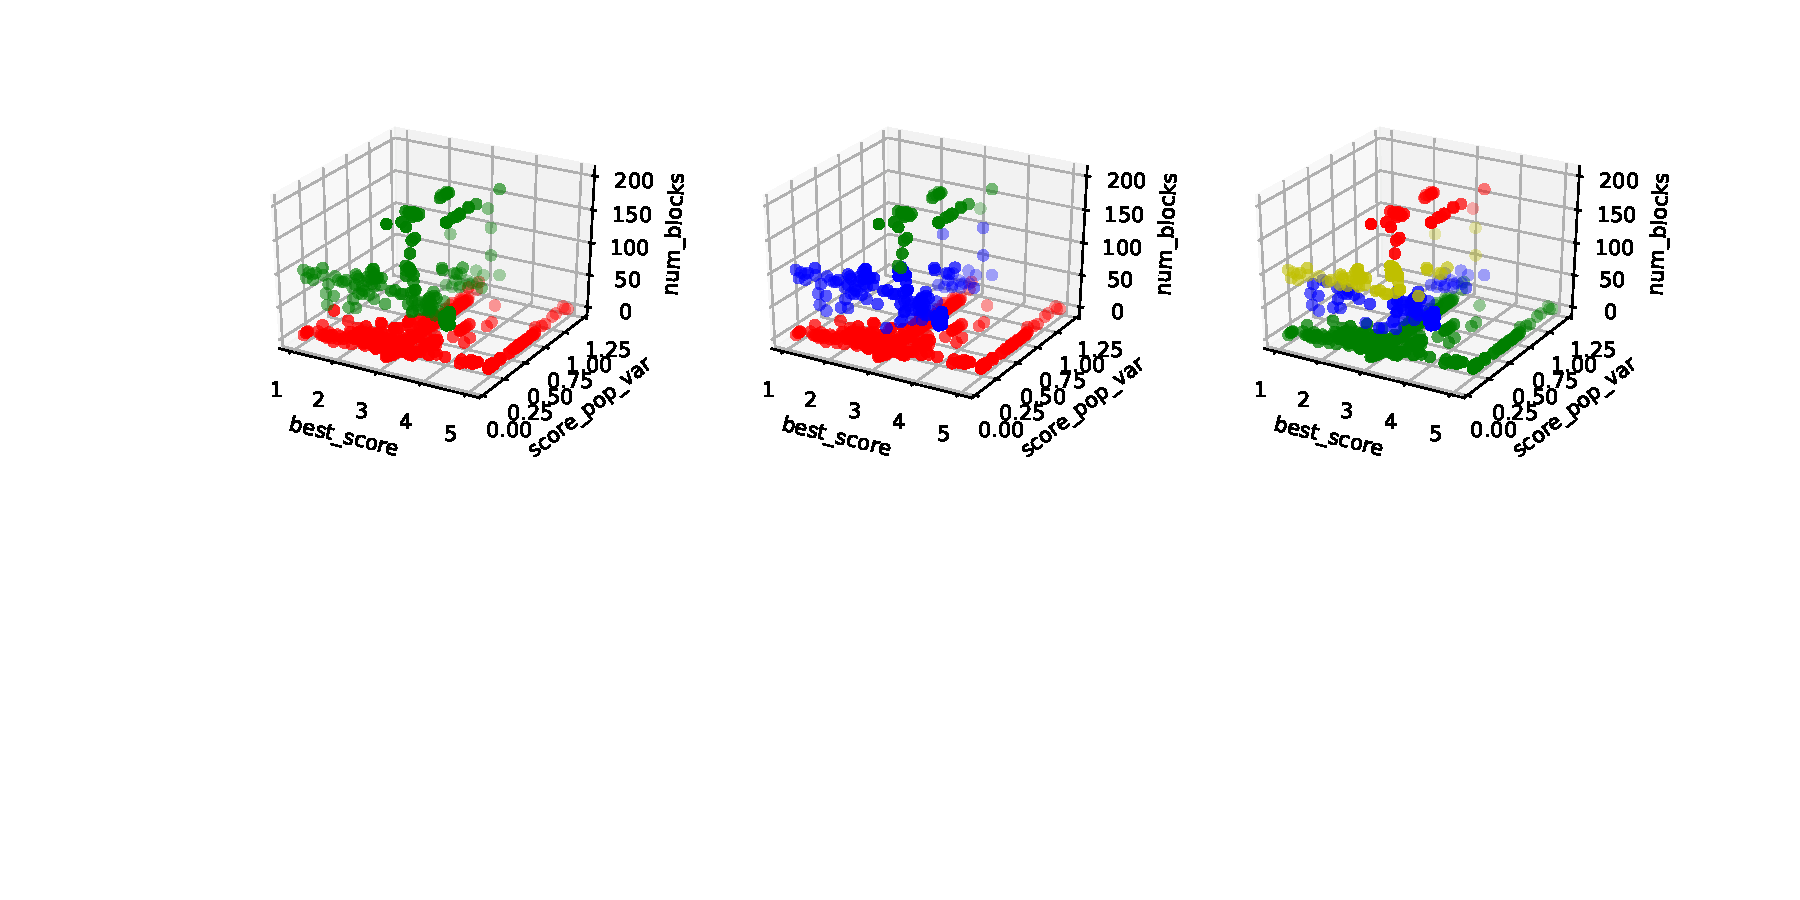
\includegraphics[width=1.0\textwidth, center]{./img/descriptive/k_means.pdf}
    \caption{K means clustering with 2,3 and 4 clusters}\label{fig:k_means}
\end{figure}

\subsection{Regression Trees}
Regression trees are a way of looking at reducing the variance of a parameter through attributes of observed instances. 
SciKit Learn has an implementation of regression trees, the code used to generate the data in this subsection is shown in Appendix code~\ref{apcode:reg_tree.py}.

Our case, we are looking at reducing the variance of the score by looking at which turns tend to cause the largest disparity in score.
To do this the algorithm look at reducing the Mean Absolute Error (MAE) of the scores, which is, in effect, reducing the $L1$ norm (sometimes referred to as the $L_1$ loss of the algorithm) of the scores.

$$\text{MAE} = \frac{1}{n}\sum_{i=0}^n |x_i-y_i|$$

Figure~\ref{fig:reg_tree} shows which moves cause the largest variance in resulting score per turn.
As you move right on the tree (or move in the false direction on the tree) then playing cooperations at the moves listed. 
The diagram backs up that by playing $C$ moves consistently (furthest right leaf) we reach a score value of $3.01$, and with 325 samples and $MAE=0.205$ this is a clear way of doing well against a large number of opponents.
If we move left on the diagram then the score value increases, which is to be expected; these are the best turns to defect and get a higher score as a result.

The move that dictates the best change in score is move $164$ (starting from the 0th turn), if we defect on this move then the score value goes up but so does the $MAE$.
Looking at leaf nodes provides an overview of solutions being grouped into minimal $MAE$ after considering 5 moves.
These represent which moves are played on the same turn by multiple solutions, all who scored approximately the same.
It is clear that there are some paths that, considering one move difference, have clusters of very different scores. 
For example, the 3rd and 4th groups from the left (with 19 and 4 members respectively) show that, on the turn $156$, you can defect and most likely get around a $3.2$ or cooperate and get half that score.
This shows that even though some solutions are similar, the corresponding opponents are vastly different in operation and will punish at some points others would forgive.

This tree does not have very many useful properties other than displaying the complexities in trying to predict a solution for any opponent.
As discussed in Section~\ref{sec:solutionGroups} if an opponent does not sit in one of the major groups it becomes incredibly hard to observe some sort of pattern between them.
One solution may be to look into combinations of initial handshakes that create the largest variation of responses in the population of opponents; from this we could map these results to a best response sequence to play for the remainder of the game.
Section~\ref{sec:follow_up} looks into this in more detail.

\begin{sidewaysfigure}
    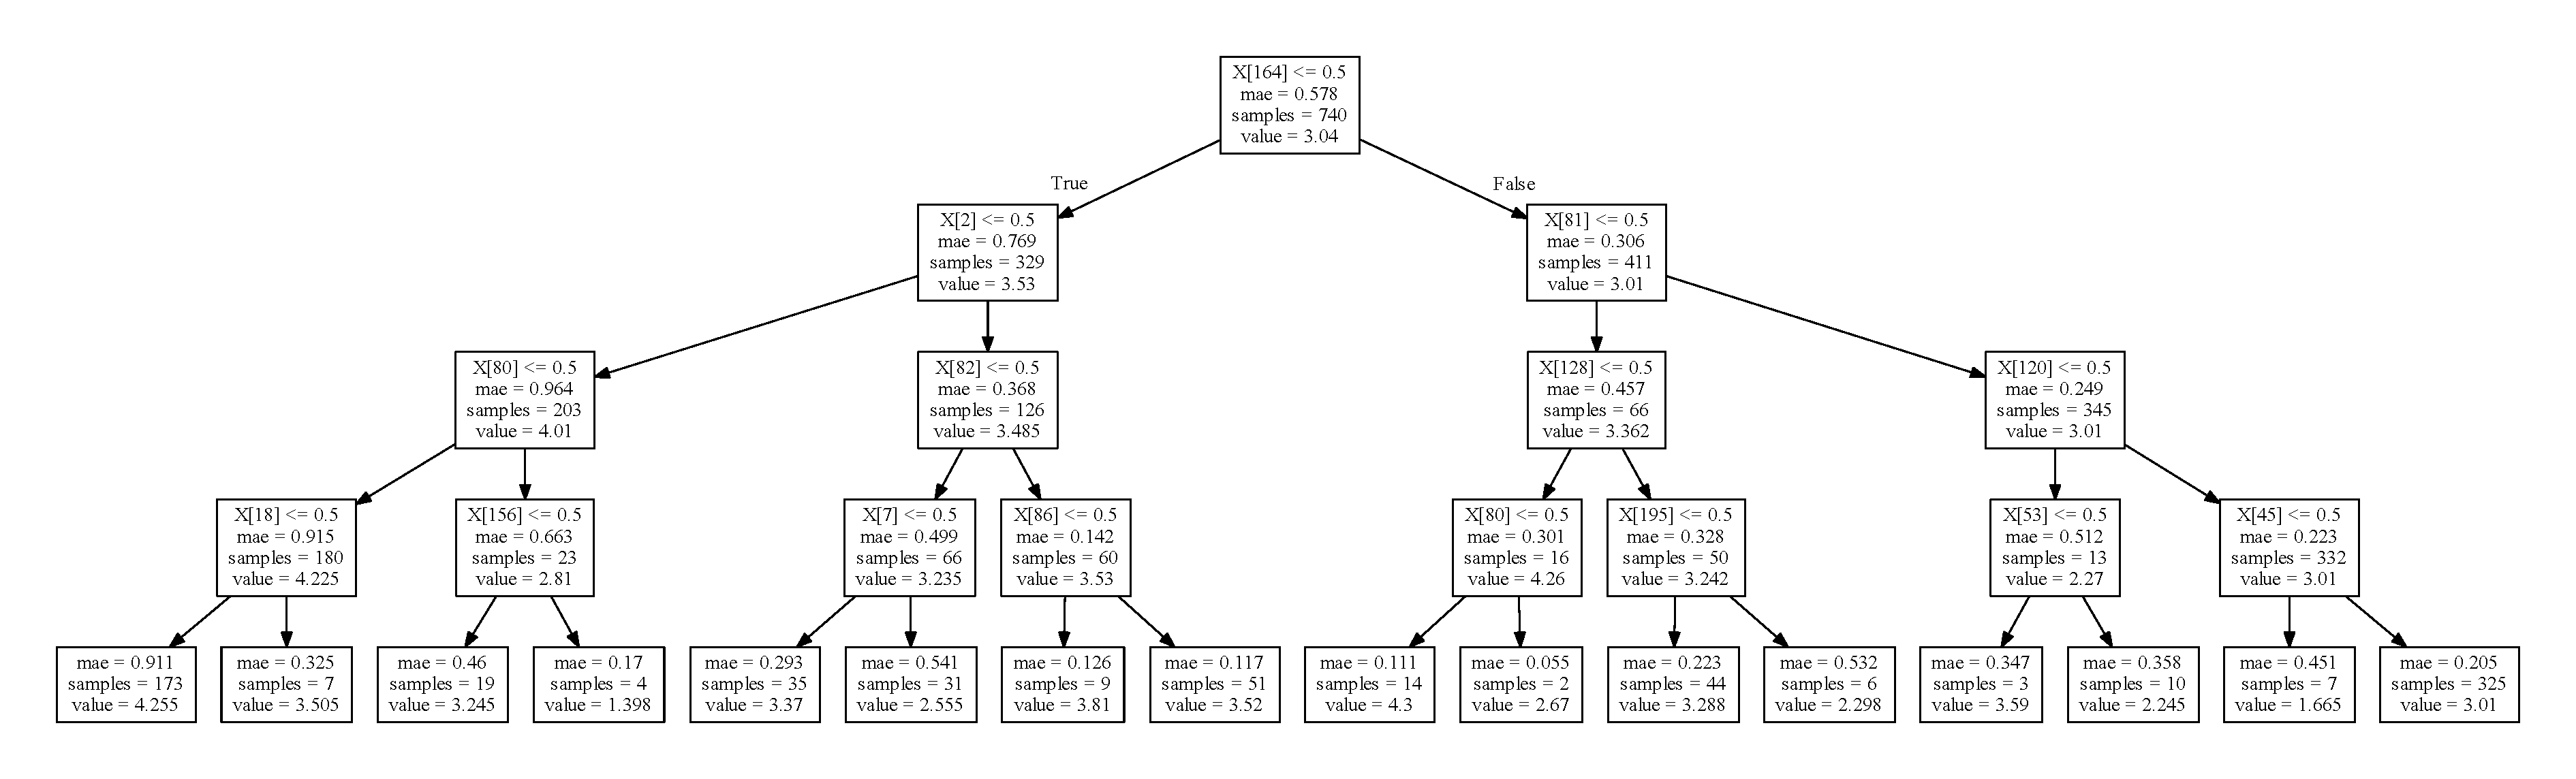
\includegraphics[width=1.0\textwidth, center]{./img/descriptive/reg_tree.pdf}
    \centering
    \caption{A regression tree showing which moves introduce the largest absolute error in the best score. If $X[i]<=0.5$ is true, it means move $i$ is a Defection move.
    \textbf{TRUE or left} $\Rightarrow D$, \textbf{FALSE or right} $\Rightarrow C$}
    \label{fig:reg_tree}
\end{sidewaysfigure}


\section{Conclusion}\label{sec:results_conclusion}
This chapter includes the most useful results from the analysis conducted on the data output.
The results are showing signs of patterns between the complexities in the solution sequence and the strategies they correspond to.
However there is no strong correlation or predictor that can be seen to allow accurate prediction of how to beat an opponent

The data produced by this report allows us to easily identify basic responses to certain predetermined tournaments.
For example, in a tournament against players Defector Hunter, Solution B1, Willing and Tricky Defector we can play $C1,199$ and easily come out on top.
The code in Appendix Section~\ref{apcode:tournCode.py} produced the results in Table~\ref{table:table_test_opsponents}.
It is clear that our solution sequence came out on top for this set of opponents, however if we played this against a different set we would score very low.
If all players in the tournament have the same solution then selecting the absolute sequence to play is trivial, however if we have multiple solutions then the problem becomes one of identifying which opponent we are playing in any round.
This problem is looked into in more detail in Section~\ref{sec:follow_up}. 

\begin{table*}
    \centering
    \begin{tabular}{ccccc}
        \toprule    
        Rank & Name & Median score & Cooperation rating & Wins \\
        \midrule
        0 & Cycler: C1,199 & 4.9625 & 0.005 & 4.0 \\ 
        1 & Tricky Defector & 2.23625 & 0.2475 & 1.5 \\ 
        2 & SolutionB1 & 1.7675 & 0.71775 & 2.0 \\ 
        3 & Defector Hunter & 1.508125 & 0.995 & 0.0 \\ 
        4 & Willing & 1.5 & 0.849 & 0.5 \\ 
        \bottomrule
    \end{tabular}
    \caption{Table of test opponents}\label{table:table_test_opsponents}
\end{table*}


The results given in this chapter represent a descriptive overview of what data we have produced.
We have looked at various methods of grouping and reducing the solutions to try and observe a clear reason for an opponent having a certain solution; yet within the data we have created there seems to be no clear sign of correlation.
If the information here is assessed further it would be beneficial to gather more data on each opponent to work with. 
The lack of usable opponent meta-data means that the GA, currently, is the only reasonable method of identifying solution sequences. 
